\chapter{bump2d}
%

% - Purpose & Problem description:
%     These first two parts give reader short details about the test case,
%     the physical phenomena involved and specify how the numerical solution will be validated
%
\section{Purpose}
The evolution of a conical dune  
is commonly used as a test case for 
two dimensional morphodynamic models. The flow is almost uniform and sub-critical.
This test case was proposed by Hudson (2005). De Vriend (1987) obtained an approximate
analytical solution for the spread angle.

%

%
\section{Description of the problem}
%
The sediment dune propagates downstream during the simulation. The formerly conical dune evolves towards a star-shaped pattern
expanding in time with a fixed spread angle. 


\subsection{Reference}

De Vriend, H.J. \textit{2DH mathematical modelling of morphological evolutions in
shallow water}. Coastal Engineering, 11(1):1 – 27, 1987.

Grass, A.J. \textit{Sediment transport by waves and currents}. Technical Report FL29,
SERC London Centre for Marine Technology, 1981.


Hudson, J. and Sweby, P.K. \textit{A high-resolution scheme for the equations
governing 2D bed-load sediment transport}. International Journal for Numerical
Methods in Fluids, 47:1085–1091, 2005.

Siviglia, A., Stecca, G.,Vanzo, Zolezzi, G., Toro, E.F., Tubino, M. \textit{Numerical modelling of two-dimensional
  morphodynamics with applications to river bars   and bifurcations}. Advances in Water Resources, February 2013. 
DOI:10.1016/j.advwatres.2012.11.010


\subsection{Physical parameters}
%
The bed load transport $QS$ is calculated with the velocities $u$ and $v$ 
using the total load formula of Grass (1981). 
There are two parameters in the formula: the constant $A_G [s^2/m]$ and the exponent $m_g$.
The first is usually obtained by experimental data and takes into account
the grain diameter and the cinematic viscosity. It is set to 0.00167 $m^2/s$ for the simulation.
The second parameter is as here usually set to $m_g=3$.
The following formula is implemented in the subroutine qsform.f:

\begin{equation}
\begin{array}{ll}
     QS = &A_G = u |u|^{(m_g-1)} \\
     QS = & A_G (u^2+v^2)  \sqrt{u^2 + v^2}
\end{array}
\end{equation}


No bottom friction, no diffusion, no porosity and no slope effect is included in the simulation.
%
\subsection{Geometry and Mesh}
%
The problem is solved in the
square computational domain [0; 1000] × [-500; 500] m using an unstructured triangle grid with 2601 nodes and
5000 elements (see figure \ref{ini}.
\begin{figure} [!h] %[!ht]
\centering
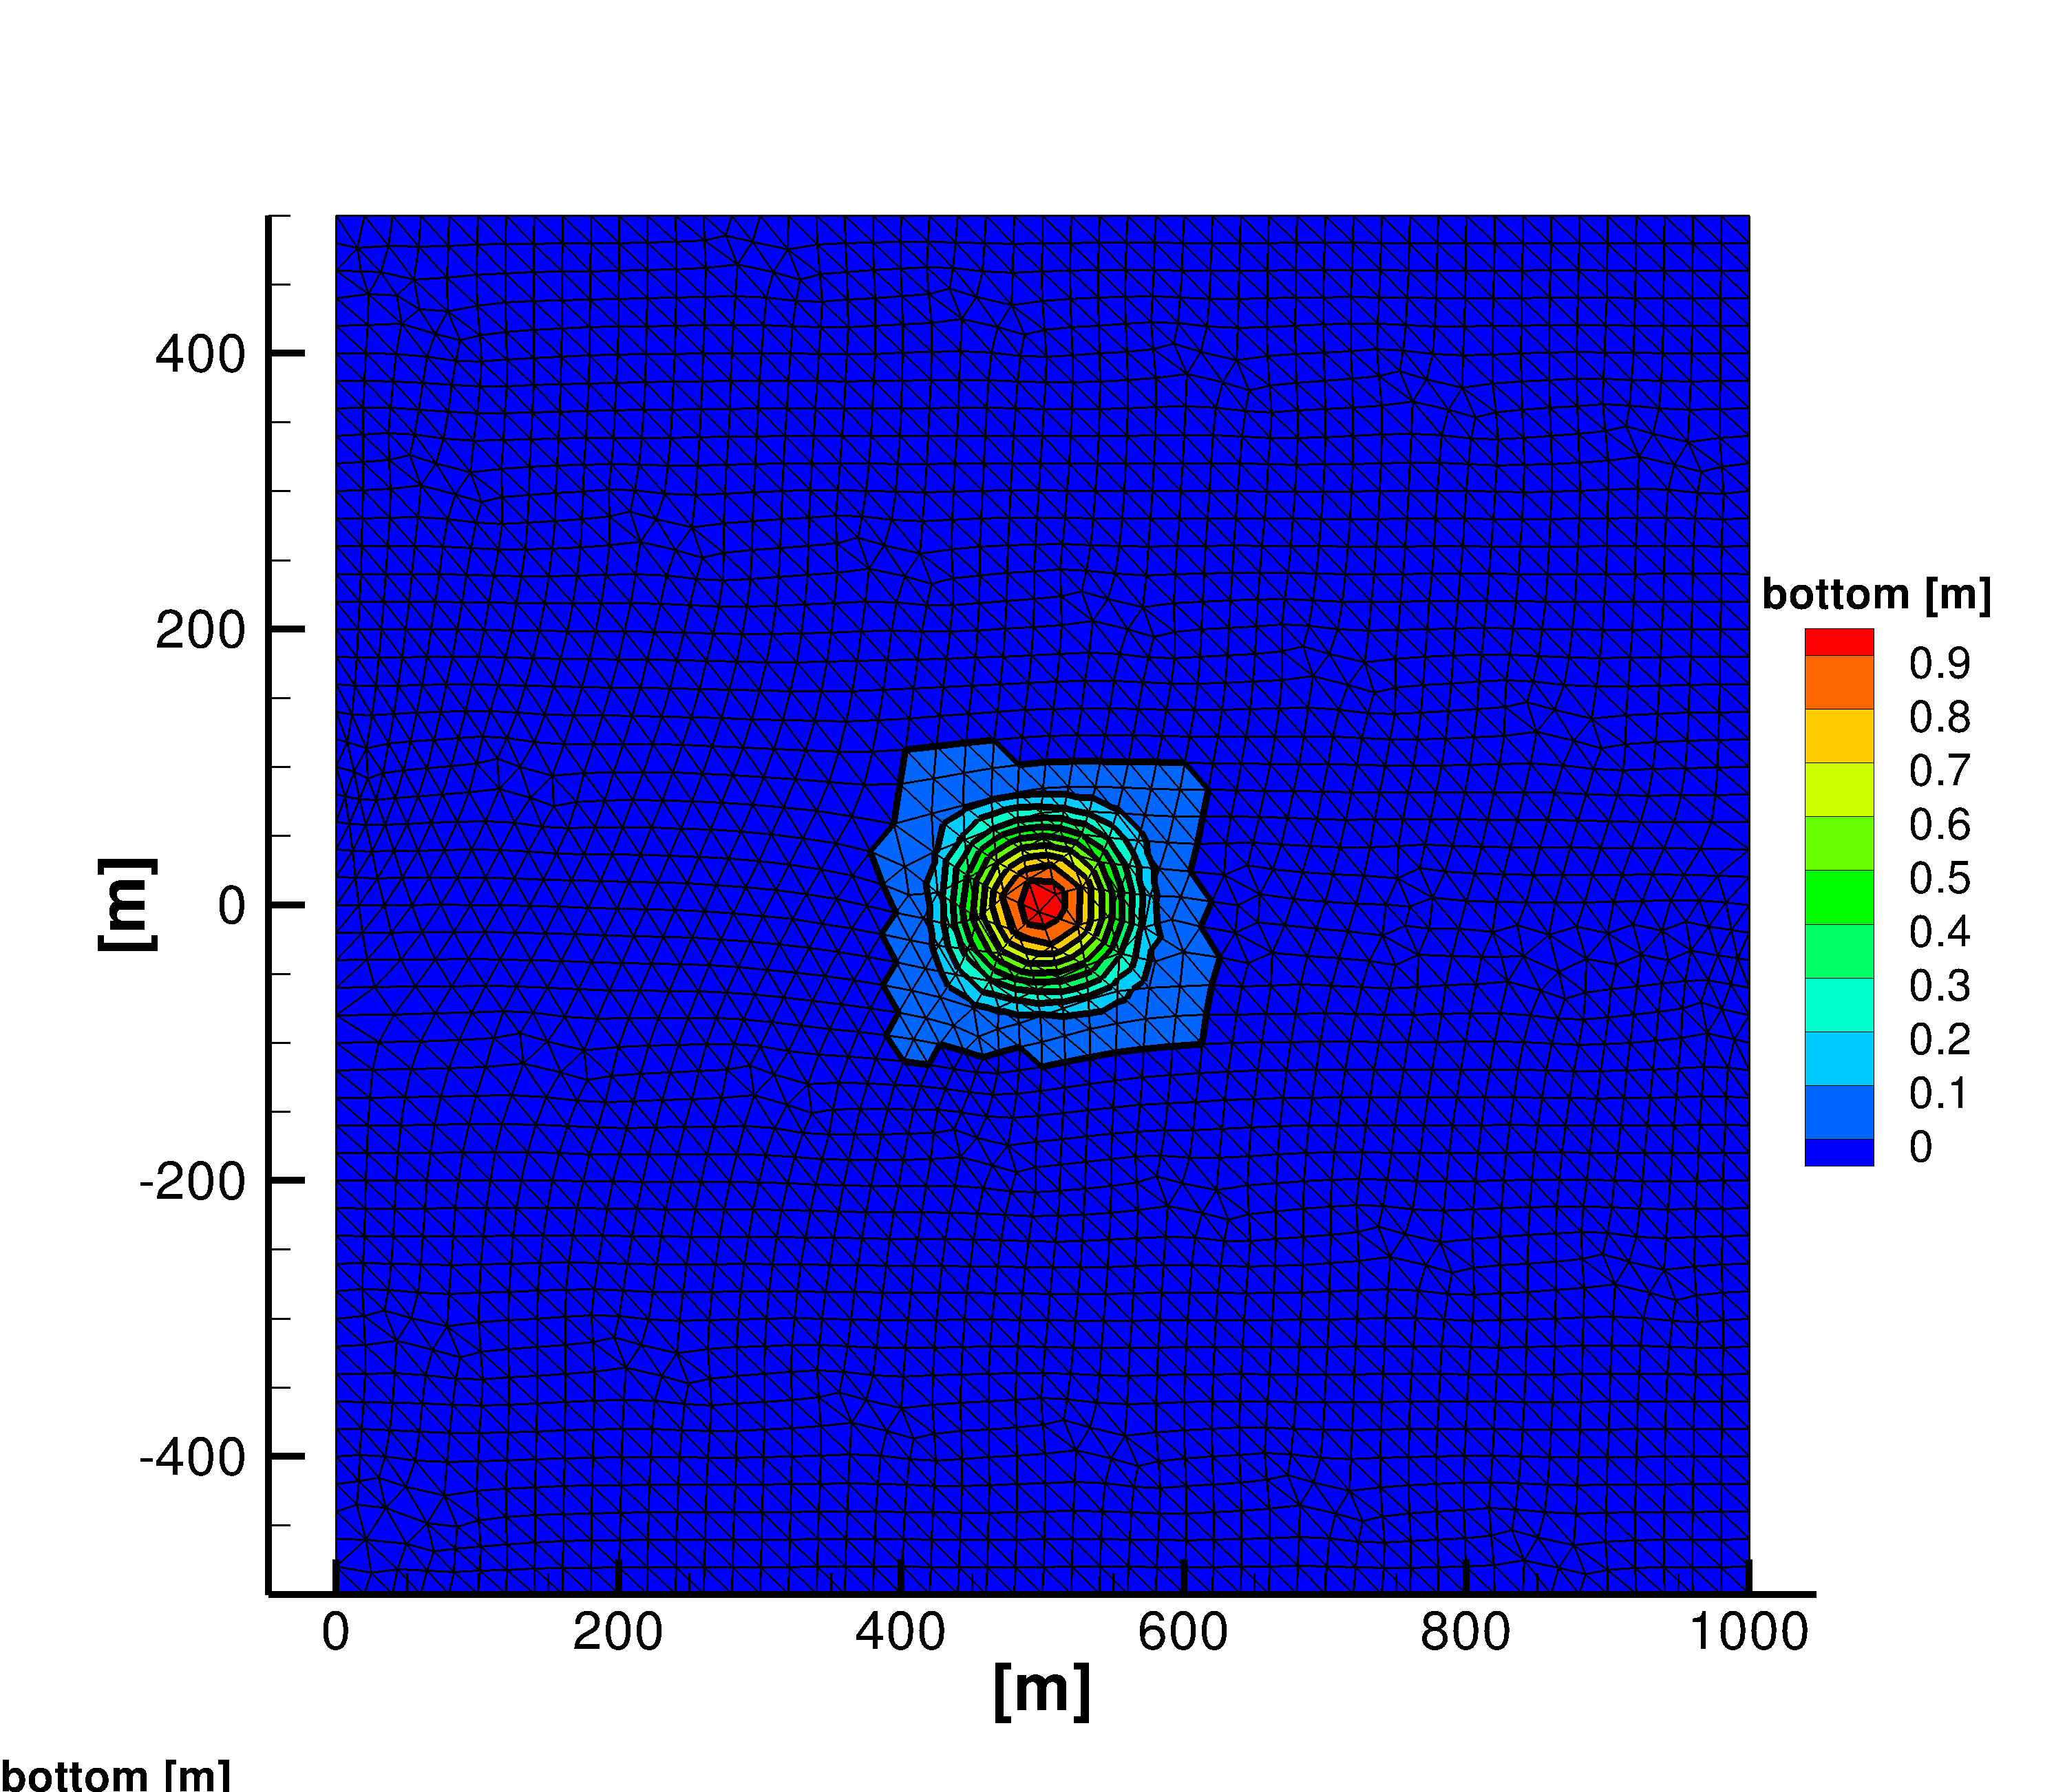
\includegraphics[width=\textwidth]{../img/sis_bump2d-ini.png}
 \caption{Simulation grid and initial bottom}\label{ini}
\end{figure}

%
\subsection{Initial and Boundary Conditions}
%
The initial condition for the
bed elevation $z$ is given by flat horizontal bed with a sediment bump:
\begin{equation}
z(x,y) = \left\{
  \begin{array}{lr}
\sin^2 (\frac{\pi (x-400)}{200}) \sin^2 (\frac{\pi (y+100)}{200}) & \text{if } x \in [400, 600] \\
& \text{and y} \in [-100,100] \\
0 & \text{otherwise} 
  \end{array}
\right.
\end{equation}

The initial condition for the hydrodynamic is the steady state computed with the following boundary conditions.
At the upstream boundary $x = 0$ a constant discharge of $Q =
1000 m^3/s$ is prescribed while a free outflow condition with a fixed water level of 10 m 
is set at the downstream boundary
x = 1000 m. At the side boundaries y = -500 and y = 500 m  a
slip condition is imposed. 
For the morphodynamic simulation only bed load transport is taken into account. There is no sediment 
input to the boundaries.


%
\subsection{Numerical parameters}
%
The time step is set to 1 s and the simulation is coupled every time step with sisyphe.


%
\section{Results}
%
The analytical solution for the spread angle $\alpha^S$
\begin{equation}
\alpha^s = \arctan (\frac{3\sqrt{3}(m_G-1)}{9m_G-1})
\end{equation}
is valid under the hypothesis of weak interaction between sediment layer
and fluid, which is ensured setting $A_G=0.00167 < 0.01$ in the Grass formula. 
With this parameters the spread angle of the analytical solution is $\alpha^s=21.787$.

The spread anlge from the simulation is calculated by using the 
0.1 m  bottom isolines after 80 h and 100h simulation time (see figure \ref{sis_bump-t2d}).
The computed spread angle $\alpha_s=25.76°$ is a little too high. With a better resolution 
spread angle will fit better to the analytical solution 
(e.g. grid with 21738 nodes and about half of the node distances $\alpha_s=23.15°$). 


\begin{figure} [!ht]
\centering
%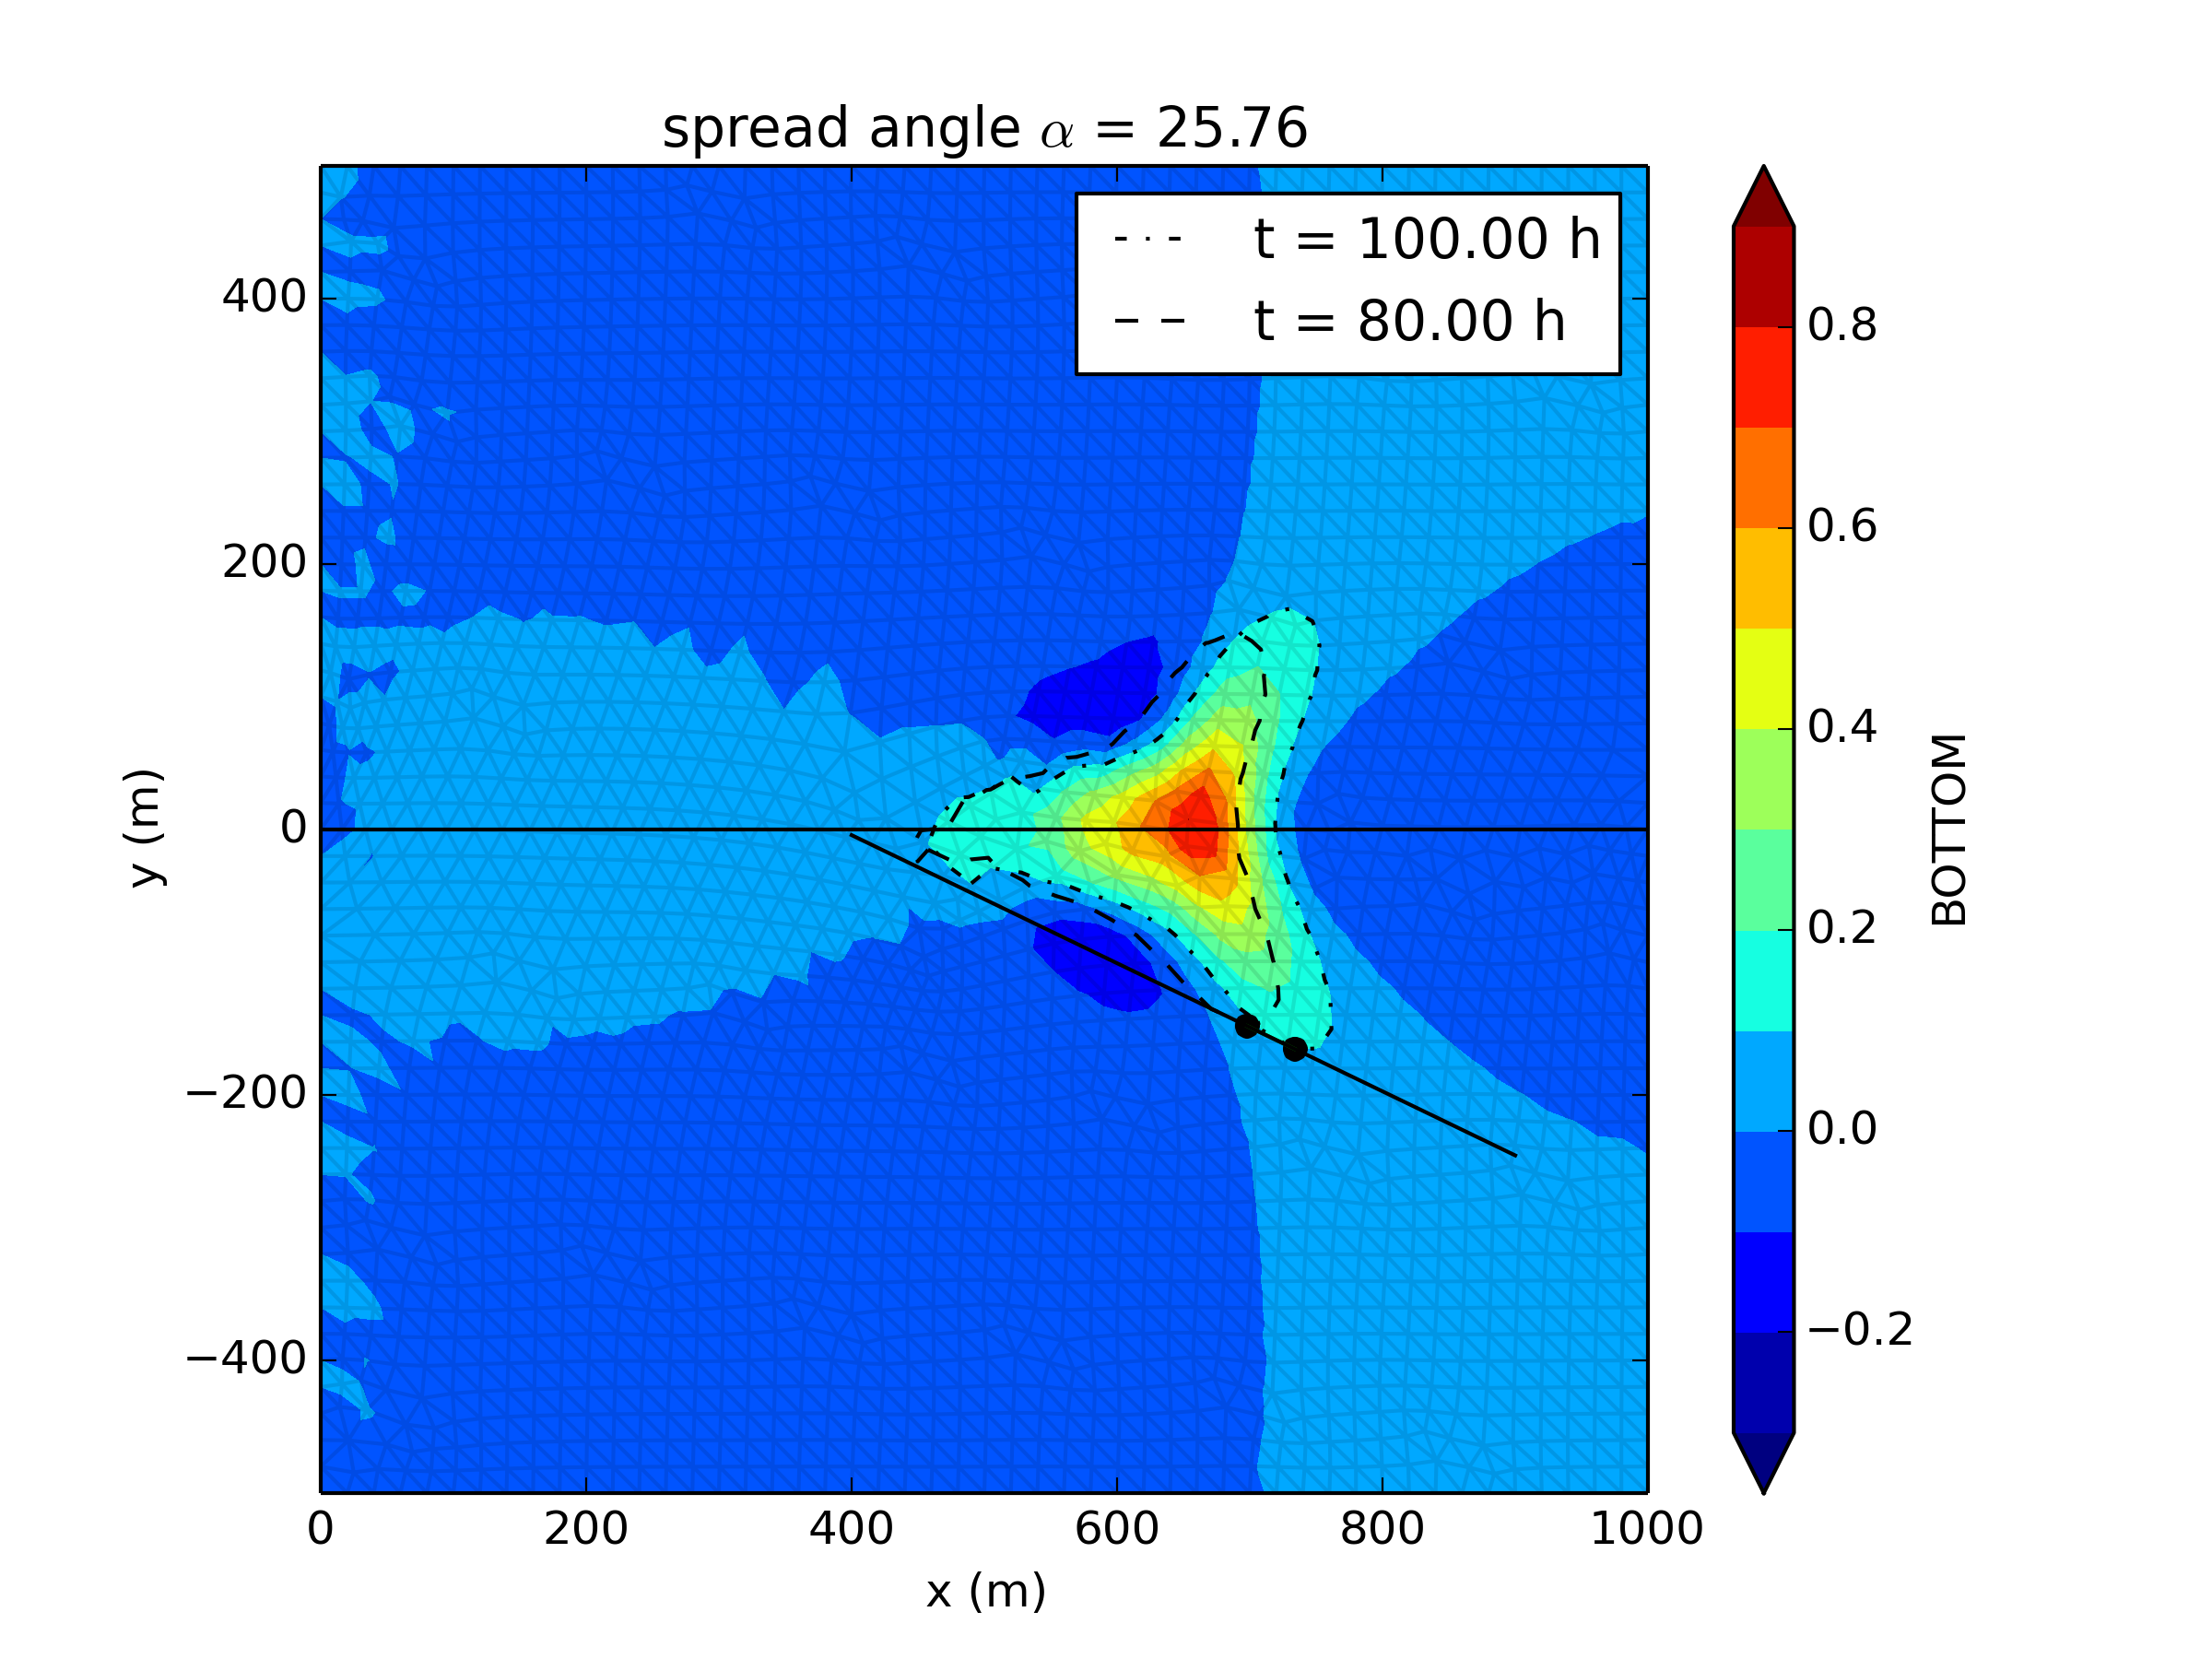
\includegraphics[scale=0.6, bb=0 0 30 30]{../img/sis_bump2d-t2d.png}
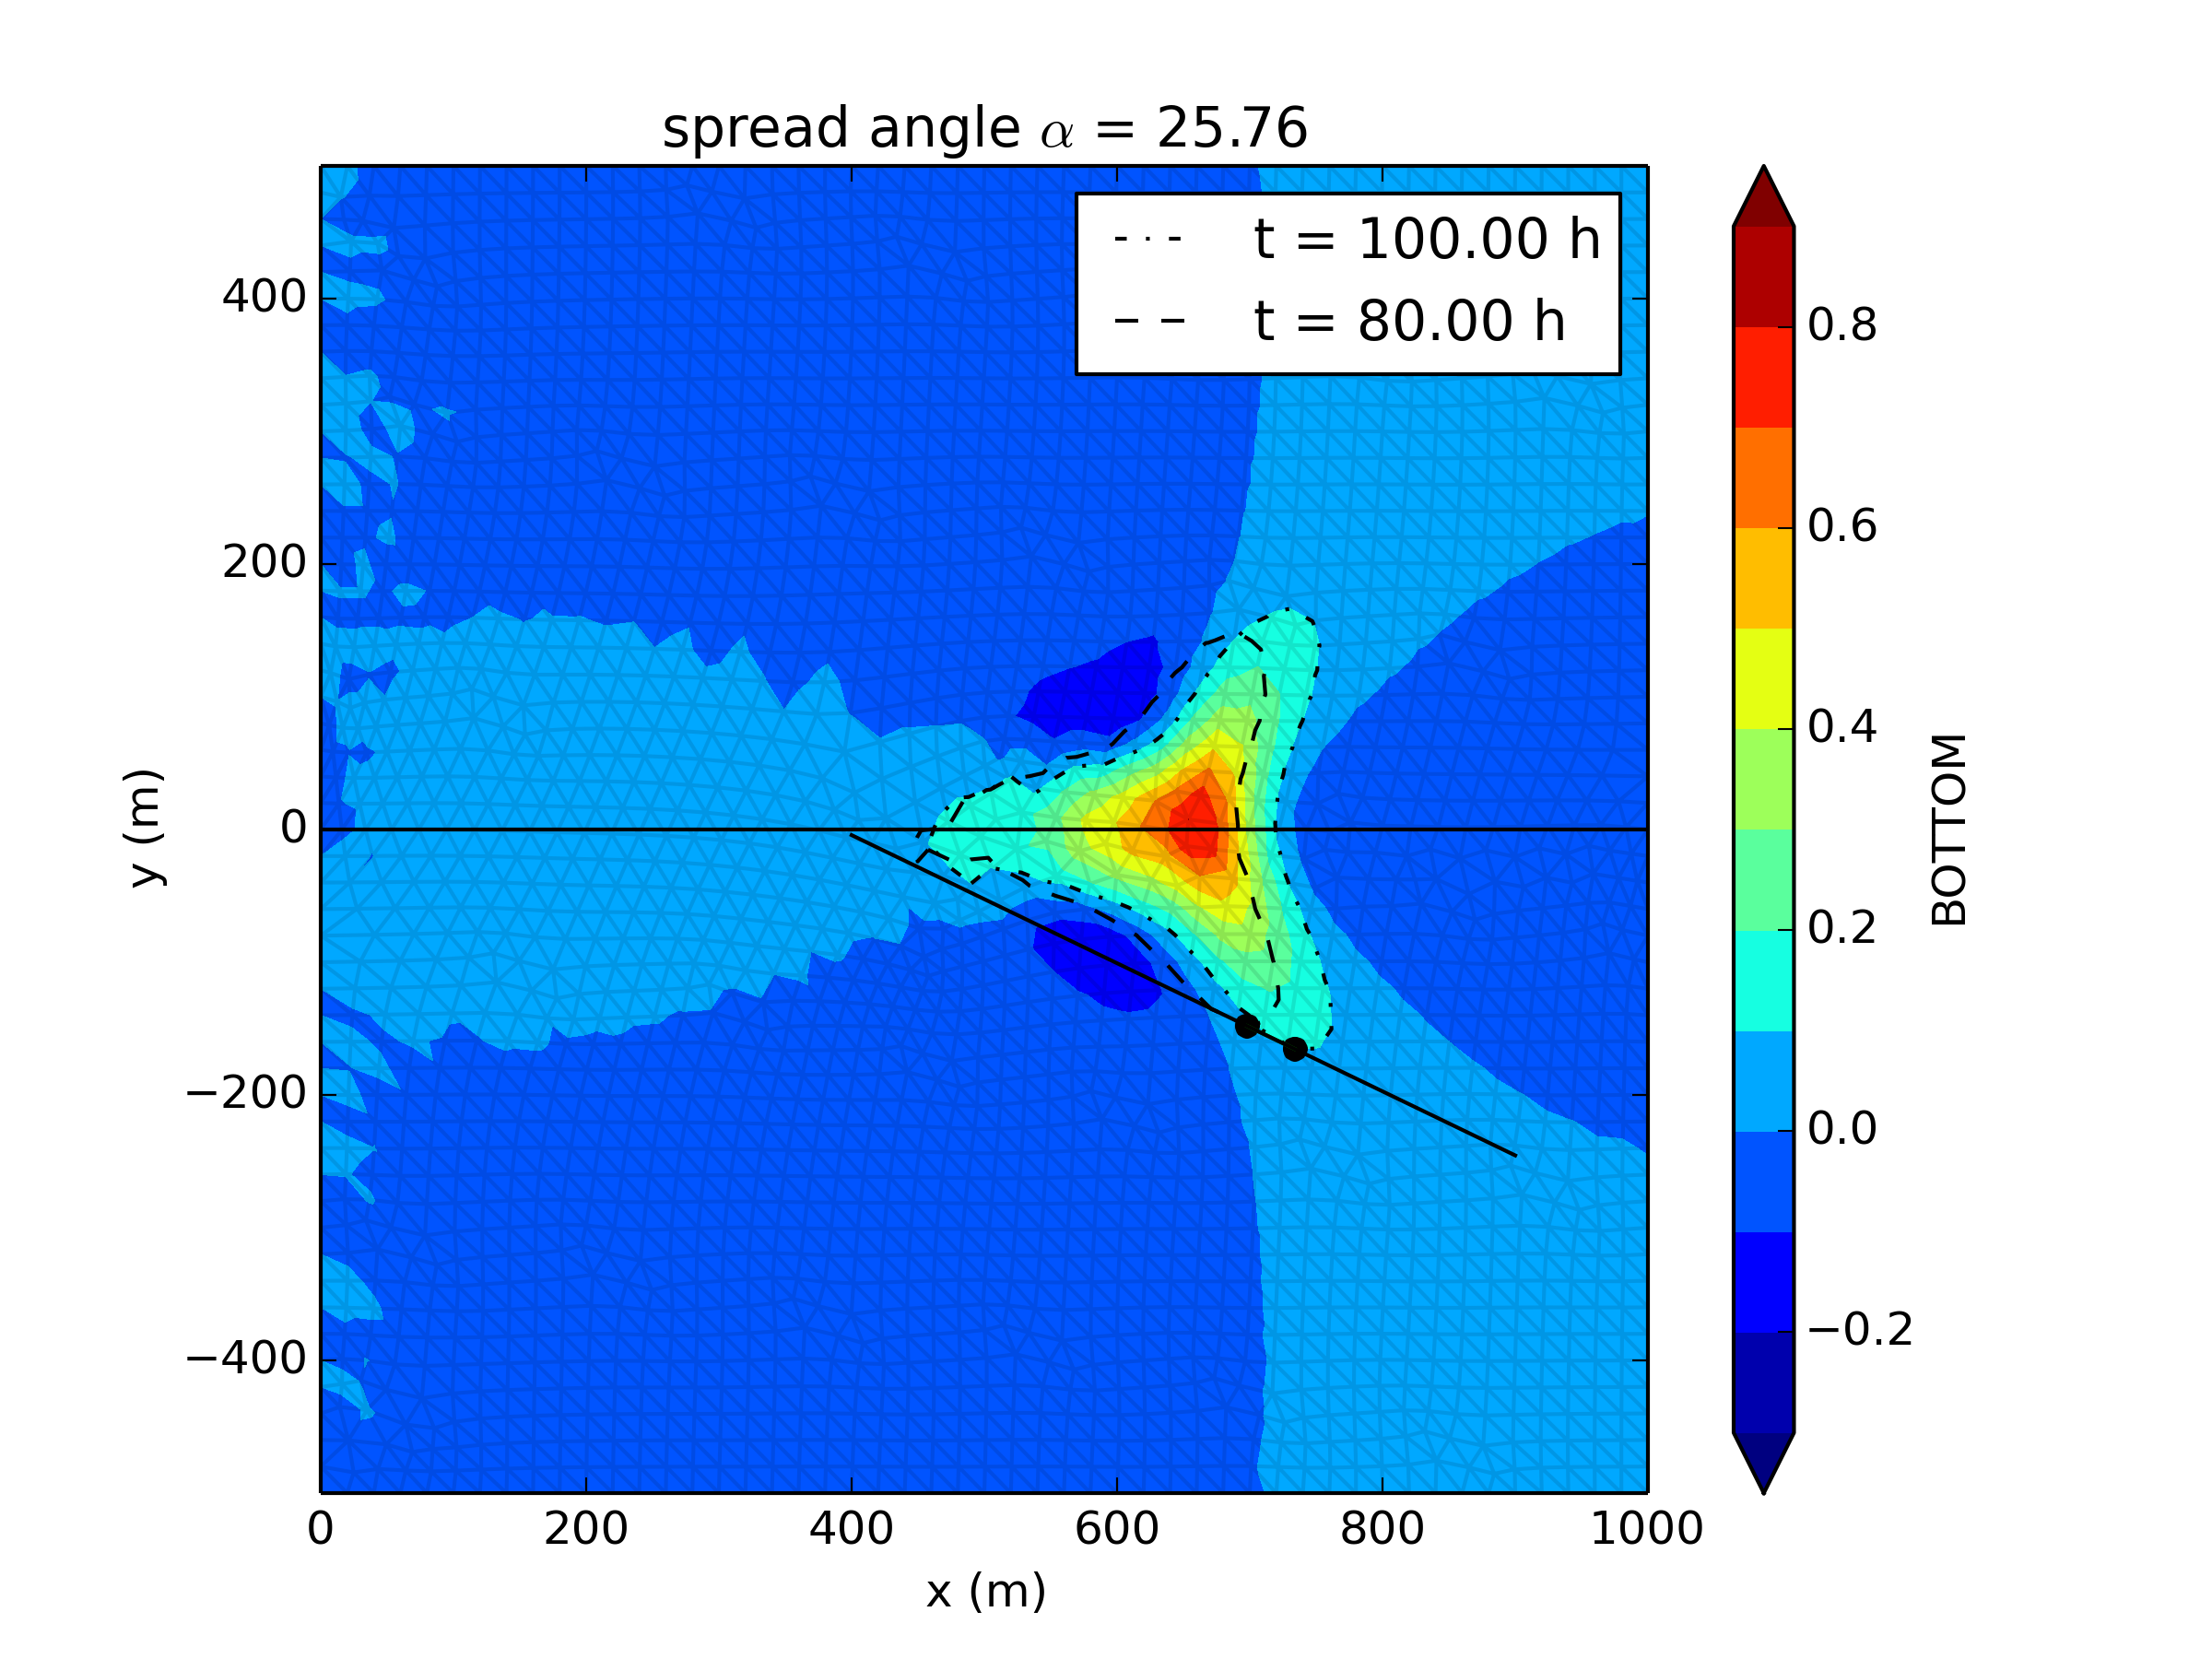
\includegraphics[scale=0.6]{../img/sis_bump2d-t2d.png}
 \caption{Simulation results after 100h}\label{sis_bump-t2d}
\end{figure}


